\subsection{Relatives Vorkommen (Referenz)
}
Ein einfacher Ansatz, der als Referenz zum Finden relevanter Wörter eines Tages dient ist der, das Auftreten jedes Tokens im Tageskorpus mit dem Auftreten im Referenzkorpus ins Verhältnis zu setzen.\\
Hierbei werden um eine Vergleichbarkeit zwischen verschiednen Tagen zu gew\"ahrleisten die Frequenzen der W\"orter \"uber die Anzahl aller Tokens im Tages bzw. Referenzkorpus normiert.\\

	\emph{Formel: } 
	\begin{equation}
	sig_{freqratio}(w) = \frac{\frac{k_{day}}{n_{day}}}{\frac{k_{2014}}{n_{2014}}}
	\end{equation}
	$k_{day}$: Frequenz des Tokens an einem Tag\\
	$n_{day}$: Summe der Frequenzen aller Tokens eines Tages\\
	$k_{2014}$: Frequenz des Tokens im Referenz Zeitrahmen (2014)\\
	$n_{day}$: Summe der Frequenzen aller Tokens im Referenzzeitraum (2014)\\
	

In Abbildung \ref{pic.rel_freq} stellt die schwarze Gerade dar, wie sich der Wert der relativen Frequenz verh\"alt, wenn die Anzahl des Auftretens eines Tokens variiert. Die senkrechte roten Linien markiert die Anzahl der Tokens, bei denen das relative Auftreten dem relativen Auftreten im Referenzkorpus entspricht. Der Wert der relativen Frequenz steigt also linear bei der Steigerung der Anzahl der Tokens eines Wortes.Dies f\"uhrt zu der Problematik der \"Ubersch\"atzung von niederfrequenten W\"orter im Referenzkorpus selbst bei relativ seltenem Auftreten im Tageskorpus. Bei niederfrequenten W\"ortern ist der Anstieg der Gerade sehr viel steiler.\\
Um diesem Problem gerecht zu werden hilft es ein Ma\ss f\"ur die Relevanz eines Wortes finden, welches ein geringe \"Uberschreitung des relativen Anteils im Referenzkorpus weniger goutiert als eine h\"ohere. Der Ansatz des Poisson Ma\ss es (\ref{subsec.poisson}) versucht dem gerecht zu werden.\\
\begin{figure}[h!]
    \centering
    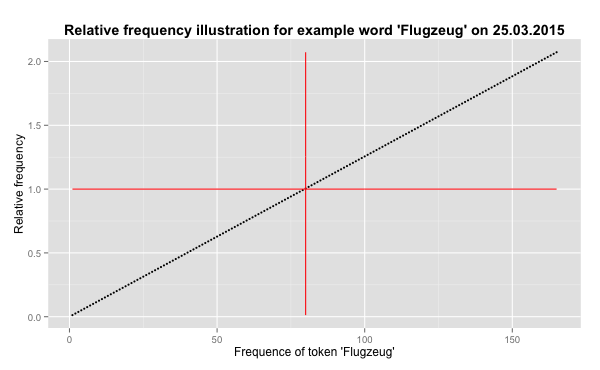
\includegraphics[width=1\textwidth]{pictures/relfreqFlugzeug.png}
    \caption{Illustration der relativen Frequenz des Tokens \enquote{Flugzeug} am 25.03.2015}\label{pic.rel_freq}
\end{figure}



\subsection{Poisson-Maß}\label{subsec.poisson}

Die Formel leitet sich aus der Poissonverteilung ab und beschreibt wie Wahrscheinlich es ist, dass die gemessene Tagesfrequenz beobachtet werden kann. 
\begin{equation}
sig_{poisson}(w) = \frac{k(\log(k)-\log(n\cdot p) -1 ))}{\log(n)}
\end{equation}
k:= Anzahl der Token von w in Tagesbericht\\
n := Anzahl der Tokens in Tagesbericht\\
p := relativer Anteil eines Tokens am Jahreskorpus\\
Es ist das gleiche Maß wie in \cite[S. 338-340]{heyer06} beschrieben und hergeleitet. Hier aber nicht zum auffinden von signifikanten Kookurenzen, sondern zum auffinden von signifikanten Nennungen im Tageskorpus gegenüber einem Vergleichskorpus.\\

\subsection{Termfrequenz inverse Dokumentenfrequenz (tf-idf)}
 \begin{equation}
sig_{tf idf}(w) = \frac{k}{\max(K)} \cdot \log ( \frac{365}{|documentdays(w)|})
\end{equation}

\subsection{Termfrequenz inverse Dokumentenfrequenz inverse Quellenfrequenz (tf-idf-isf)}
\emph{Idee: } W\"orter sind dann interessant, wenn sie an einem Tag in m;glichst vielen verschiedenen Quellen gennant werden.\\
Als Quelle definieren wir die Serveradresse einer Quelle. Diese wird mittels eines regul\"aren Ausdrucks aus den zugeordneten Quellen in der MySQL-Datenbank ermittelt. Als Gesamtzahl der Quellen verwenden wir alle an einem Tag den W\"ortern zugeordnete Quellen.\\
Das entstandene Signifikanzma\ss wird wie folgt definiert:
 \begin{equation}
sig_{tf idf isf}(w) = sig_{tf idf}(w) \cdot \log ( \frac{Q_d}{q_d(w)})
\end{equation}
Analog zur inversen Dokumentenfrequenz wird also das tf-idf-Signifikanzma\ss  mit dem Logarithmus der inversen relativen Anzahl der Quellenfrequenz multipliziert. $Q_d$ ist die Anzahl aller erw\"ahnten Quellen an einem Tag $d$ und $q_d()$ bildet ein Wort auf die Anzahl der Quellen ab, in denen das Wort an Tag $d$  erw\"ahnt wird. 
